% !TEX root = ../thesis.tex
\section{Vytvoření řečového korpusu EL promluv}
\label{chap:construction:corpus}

Před započetím libovolných prací na vytvoření ASR systému pracující s lidmi po TL je potřeba vytvořit řečový korpus, který poslouží k natrénování a otestování vytvořeného systému. Tato data jsou velmi specifická a je proto potřeba zajictit co možná největší množství kvalitních\footnote{Kvalitou je myšlena věrnost dat dané doméně, dále se mluví o přesnosti ve smyslu bezchybnosti přepisů.} a přesných dat, které budou součástí řečového korpusu.

V části \ref{chap:cause:desease} bylo zmíněno, že ročně se objeví více než 100 nových případů trvalé ztrázy hlasu ročně. V \cite{Skvrnakova2010} bylo řečeno, že více rizikovými osobami jsou starší lidé, kteří intenzivně kouří a konzumují alkohol. Přesto je patrný trend snižujícího se věku pacientů a s tím související nárůst případů ztráty hlasu. Přičteme-li již zmíněný psychologický aspekt jeho ztráty, je zřejmé, jak komplikované je získat ke spolupráci i jen jednoho řečníka ochotného podstoupit naročné\footnote{I pro zdravého člověka je někdy někalikahodinové nahrávání vysilující. Pro jedince po TL to je z mnoha důvodů ještě řádově náročnější.} nahrávání.

Při libovolné práci s pacienty po TL, dřív nebo později dojde k určité formě spolupráce s oddělením ORL, které má nastarosti péči o tyto pacienty. V našem připadě nejprve s ORL klinikou při Fakultní nemocnici v Plzni a poté i s ORL klinikou Fakultní nemocnice v Motole. S jejich pomocí jsme získali ke spolupráci jednoho řečníka. Konkrétně se jedná o dámu v duchodovém věku, která podstoupila TL před více než 15 lety. Po překonání ostychu\footnote{Podle jejích vlastních slov nebyla schopna několik let po operaci ani zvednout nečekaný telefonní hovor, natož mluvit na veřejnosti.} se byla schopna naplno vrátit do běžného života a dokonce v určité formě opět přednášet o stomatologii na Lekařské fakultě v Plzni Univerzity Karlovy.

S její pomocí jsem, v 1. etapě nahrávání, byli schopni pořídit přes 10 hodin promluv, viz tab. \ref{tab:construction:recording}. Nahrávání probíhala v relativně spartánských podmínkách za plného provozu katedry. Přesto získaná data neobsahují žádný nežadoucí ruch, kromě toho produkovaného samotným EL.

Nahravací aparatůra sestávala z miniaturního profesionálního mikrofonu (DPA d:screet 4061-FM), zesilovačem (DPA MMA6000), externí zvukové karty a běžného notebooku. Mikrofon byl pomocí bezpolštářkové náplasti přilepen poblíž pravého koutku úst, aby zaznamenaná řeč měla co možná nejvyšší kvalitu.

Celé nahrávání bylo v 1. etapě rozděleno do 14 samostatných sezení a probíhalo od prosince roku 2010 do května roku 2011. Každé sezení trvalo přibližně dvě hodiny, během kterých se podařilo získat necelou hodinu akustických dat. Samotné nahrávání se sestávalo z 10 - 20 minutového úseku nahrávání a přibližně 10 minut dlouhého odpočinku. Ten byl nezbytný hlavně z důvodu únavy řečníka.

Před samotným nahrávánám byly, z databáze obsahující stovky tisíc vět, pečlivě vybrány a vytvořeny 2 sady vět:

\begin{enumerate}
  \item sada obsahující všechny možné české fonémy - \textit{40 vět}.
  \item sada obsahující věty s reálnou četností fonémů - \textit{5000 vět} \cite{Radova2000}.
\end{enumerate}

\noindent Pořízené nahrávky vždy odpovídají 10 - 20 minutovému úseku nepřerušovaného nahrávání. Výsledné soubory vždy obsahují několik vět. Ty jsou od sebe odděleny minimálně 5 sekundovým úsekem ticha. Nahrávky dále mouhou obsahovat opakování chybně vyslovené věty, přeřeknutí, kýchnutí a další neřečové události. Z tohoto důvodu bylo nezbytné pořízené nahrávky anotovat, přestože byly pořízené na základě připravené sady vět.

Ještě před samotným anotováním byly nahrávky, podle úseků s tichem, rozsekány na menší části. V tomto případě úplně dobře nefungovaly\footnote{Problémem byl zvuk EL, se kterým nebylo při návrhu VAD počítáno.} standardně používané sofistikovanější metody pro voice activity detection (angl. zkratka VAD), a proto bylo využito principu energie. Pro každou nahrávku obsahující více vět se pomocí vzorce

\begin{equation}
  \label{eq:construction:energy}
  E_{RMS}(n) = \sqrt{\frac{1}{N} \sum_{n=1}^{N} \left| x(n) \right|^2},
\end{equation}

\noindent kde $N$ představuje počet vzorků v nahrávce a $x(n)$ představuje pravoúhlé okénko vzorku $n$. Pro tento případ se ukázalo jako vhodnější volit root-mean-square energy ($E_{RMS}$) a empericky se ukázalo, že vhodná délka okénka je v rozmezí $10 - 100$ ms. Na obr. \ref{fig:construction:el_speech} je zobrazena podoba audio signálu a spektrogram promluvy \textit{\uv{Akcie Komerční banky}}. Zároveň je zde vypočtené hodnoty energie a celková průměrná energie. Tyto hodntoty slouží pro určení míst kde začíná a končí věta. Na začátku a konci každého úseku je vhodné mít minimálně $0.5$ s ticha, aby bylo zajištěna správná funce výsledného ASR systému, viz \ref{chap:asr:parametrization}. Tím pádem, pokud energie nějakého úseku $x$ je $E_{RMS}(x) < avg(E_{RMS})$ a zároveň délka tohoto úseku $dur(x) \geq 1\ [s]$, tak je možné nahrávku v tomto úseku rozdělit.

\begin{figure}[hbpt]
  \centering
  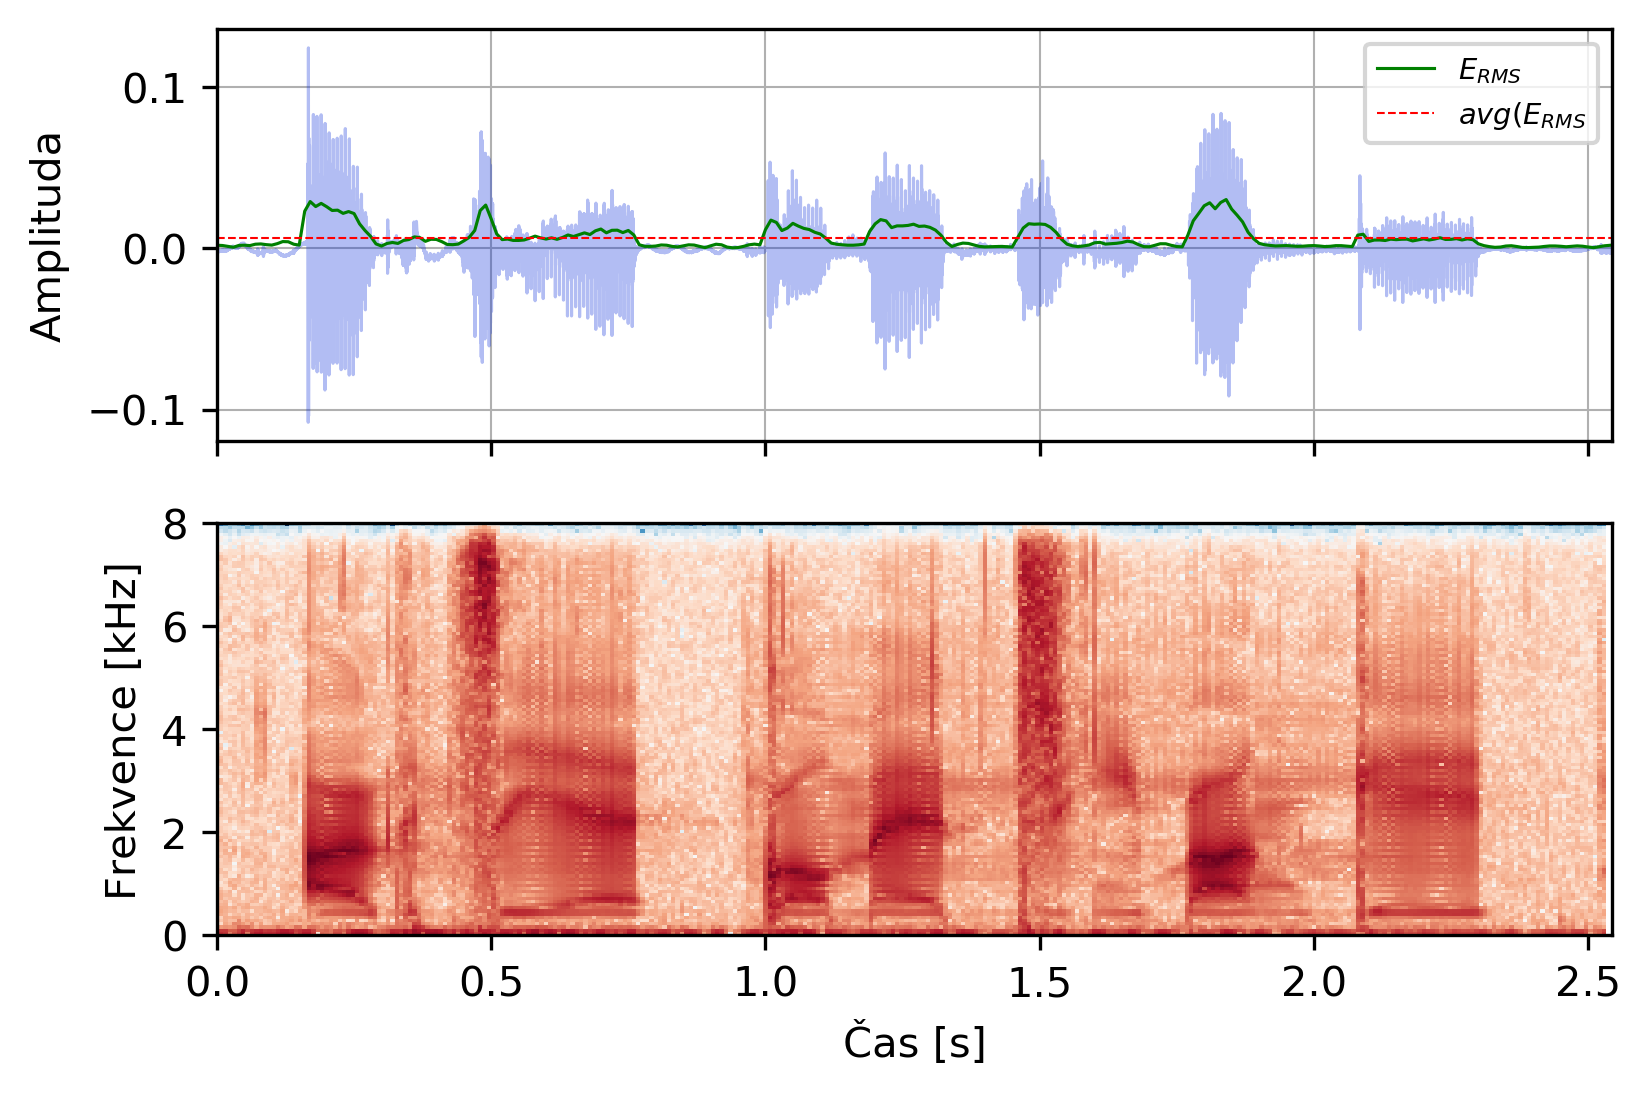
\includegraphics[width=0.9\textwidth]{./ch5-construction/img/energy_spec_el.png}
  \caption{Průběh a spektrogram promluvy a vyznačenou energií EL promluvy.}
  \label{fig:construction:el_speech}
\end{figure}

Pokud řečník v průběhu věty z libovolného důvodu udělal pauzu větší než $1\ s$, tak v důsledku výše popsaného postupu byla věta rozdělena na dvě části. Nejedná se však o významný problém, protože výsledné kratší useky jsou anotovány. Při vytváření ASR systému není podstatné zda promluva představuje celou větu, ale spíše to jestli je tento úsek správně přepsán. Fakt, že některé věty jsou rozděleny je důvodem proč v tab. \ref{tab:construction:recording} je více souborů než vět.

K anotaci posloužil interní anotační nástroj a podíleli se na ní celkem 3 anotátoři z řad studentů. Přepis jednoho anotátora, byl vždy zkontrolován jiným anotátorem. Ačkoli bylo potřeba přepsat relativně malé množství dat (cca 10 hodin audio záznamu), tak anotace všech promluv zabrala přibližně 2 měsice. Hlavním důvodem byla relativně dlouhá doba, po kterou se anotátoři adaptovali na specificka EL řeči. Hlavně ze začátku nebyli schopni poruzumnět obsahu promluvy a tím pádem jej správně přepsat. To významně prodloužilo dobu potřebnou k anotaci celého řečového korpusu.

Pokud je k produkci řeči použit elektrolarynx, tak vedlejším produktem je nezanedbatelný ruch způsobený samotným zařízením, viz část \ref{chap:cause:treatment:foniatric}. Přeci jen jeho jedinout funkcí je vybudit vzduch v dutině ústní a tím umožnit produkci slyšitelné řeči. Z tohoto důvodu byly v průběhu anotace ignorovány v podstatě všechny skupiny neřečových událostí, protože vetšina nahrávek by byla anotována jako, že obsahují šum.

Výsledný řečový korpus představuje $5040$ unikátních vět rozdělených do $6385$ souborů (viz tab. \ref{tab:construction:recording}), které v průměru obsahují $7$ slov o průmerné délce $5$ znaků. Tento korpus slouží jako základ pro všechny budoucí experimenty.

\begin{table}[htpb]
  \centering
  \def\arraystretch{1.5}
  \pgfplotstabletypeset[
    col sep=comma,
    string type,
    columns/phase/.style={column name={Nahrávání}, column type={l}},
    columns/length/.style={column name={Délka \textit{[HH:MM:SS]}}, column type={r}},
    columns/sentences/.style={column name={Počet vět}, column type={r}},
    columns/files/.style={column name={Počet souborů}, column type={r}},
    every head row/.style={
      after row={
        \cmidrule(r){1-1}
        \cmidrule(lr){2-2}
        \cmidrule(lr){3-3}
        \cmidrule(l){4-4}
      },
      before row={\toprule}
    },
    every last row/.style={after row={\bottomrule}},
  ]{./ch5-construction/tabs/02-recording1-stats.csv}
  \caption{Informace o korpusu nahrávek z 1. etapy nahravání.}
  \label{tab:construction:recording}
\end{table}
